\section{Lecture 4: 02/03/2021}
Today we will be talking about sets! As you go forward in math, you will repeatedly see the fundamentalness of sets. Here are some sets you may be familiar with:
\begin{itemize}
    \item $\N$ which is the set of natural numers (positive integers)
    \item $\Z$ which is the set of integers
    \item $\Q$ which is the set of rational numbers
    \item $\R$ which is the set of real numbers
    \item $\C$ which is the set of complex numbers
\end{itemize}
\subsection{Some Notation}
There are two ``flavors" of notation for specifying a set.
\begin{enumerate}
    \item The first is when we want to apply a condition. This takes the form of 
    $$
    \{w \in \Z \mid 3 \le w < 6 \} = \{3, 4, 5\}
    $$
    where $\mid$ means ``such that".
    \item Another form of notation looks like
    $$
    \left\{\frac{1}{k} \mid k \in \Z\right\}
    $$
\end{enumerate}
The difference between these two is the order of the variable. In the first we have $\{\text{variable} \; \mid \text{condition}$ and in the second we have a the variable and then the relation. 
\begin{example}
True or false. 
\begin{enumerate}
    \item $\{n \in \Z : 2 \mid n \} = \{2k : k \in \Z \}$ We see that this is true as both sides are the even integers.
    \item $\{2n \mid n \in \Z\} = \{-2n \mid n \in \Z\}$ These are again both describing even integers so the equality holds.
\end{enumerate}
\end{example}
\subsection{Set Operations}
Before talking about set operations, it is important to go over a particular set relation. We can draw the intuition for this from our knowledge of Venn diagrams. This is made more clear in the figure \ref{fig:sets}.
\begin{figure}[h]
    \centering
    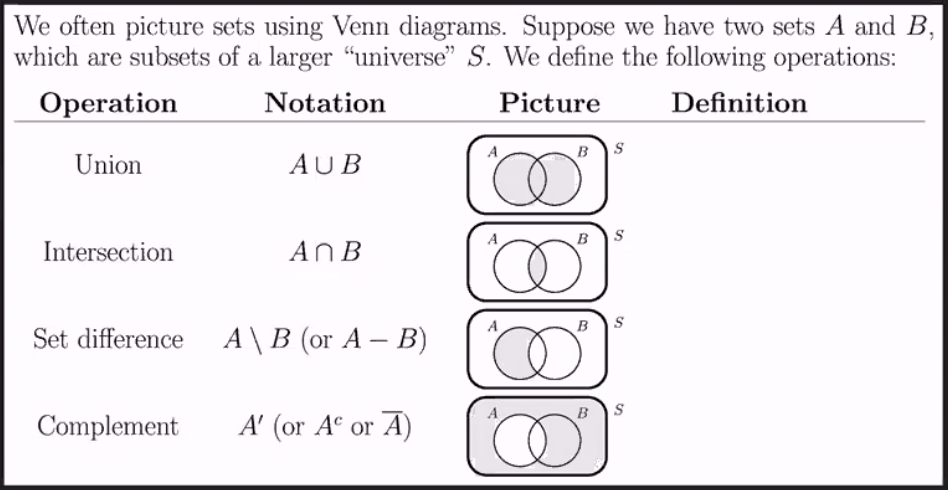
\includegraphics[scale=.4]{notes/images/set-relations.PNG}
    \caption{Set Relations as Venn Diagrams}
    \label{fig:sets}
\end{figure}
Filling in the definitions for Figure \ref{fig:sets} we have:
\begin{enumerate}
    \item $\{x \mid x \in A \; \text{or} \; x \in B\}$
    \item $\{x \mid x \in A \; \text{and} \; x \in B\}$
    \item $\{x \in A \mid x \not\in B\}$
    \item $\{S\setminus A\} = \{x \in S \mid x \not\in A\}$
\end{enumerate}
If we want to prove $x \in A \cap B$, show $x \in A$ and $x \in B$.
\begin{definition}
Let $S, T$ be sets. We say $S$ is a \textit{subset} of $T$, written $S \subseteq T$, if every element of $S$ is also an element of $T$. We say $S$ is a proper subset of $T$, $S \subsetneq T$, if $S \subseteq T$ and $S \neq T$. 
\end{definition}
\subsubsection{Interesting Question!}
Is the empty set an element of every set? We can parse this question as : If $x \in \phi$, is $x \in S$. We can think of a similar (perhaps not obviously related) question. If a person is drinking alcohol, they must be $\geq 21$. This statement has a counterexample as we can find a counterexample (a 19 year old drinking alcohol). Turning back to our original question, we see that $x \in \phi$ is always false. Therefore, we have that the statement itself holds. When things are true for this reason, we say that things are \textit{vacuously} true. This means that the antecedent (in this case $x \in \phi$ can never be satisfied. 
\subsection{Set Inclusion}
Consider the following example,
\begin{example}
Let $A = \{12n \mid n \in \Z\}, B = \{k \in \Z \mid k \; \text{is even}\}\text{, and } C = \{3j \mid j \in \Z\}$. Prove using the definitions of subset and intersection that $A \subseteq B \cap C$. 
\begin{proof}
Let $x \in A$. Then, $x = 12n$ for some $n\in \Z$. We can rewrite $x = 2(6n)$, so $x$ is even sine $6n \in \Z$ so $x\in B$. We can also rewrite $x = 3(4n)$, so x $\in C$. By definition of intersection, $x \in B \cap C$.
\end{proof}
\end{example}
\subsection{Set Equality}
In proving set equality, we rely on the fact that if the left is a subset of the right and vice versa, then our sets are equal. To further show this, we consider the following example.
\begin{example}
$(A \cap B) \cup (A \setminus B) = A$
\begin{proof}
Proving the first inclusion $(\subseteq)$, let $x \in (A \cap B) \cup (A \setminus B)$. By the definition of the union, we have that $x \in A \cap B$ or $x \in A \setminus B$. In either case, $x \in A$ relying on the definition of the the intersection and set difference. 
\smallbreak
Now we need to prove the other direction $\supseteq$. Let $x \in A$. Either $x \in B$ or $x \not \in B$.
\begin{itemize}
    \item If $x \in B$, then $x \in A \cap B$. 
    \item If $x \not\in B$, then $x \in A \setminus B$.
\end{itemize}
In either case, $x$ is in the union of $(A \cap B)$ and $(A \setminus B$ by definition of the union.
\end{proof}
\end{example}
\subsection{The Cartesian Product}
Unlike our other set relations, Venn diagrams don't work well for visualizing the Cartesian product. We define the Cartesian product as
\begin{definition}
The \emph{Cartesian product} $Z$ is the product of two sets $X, Y$ such that the set $Z$ contains all ordered pairs $(x, y)$ for which $x \in X$ and $y \in Y$. 
\end{definition}
\subsection{The Power Set}
Here is one more definition!
\begin{definition}
If $S$ is a set, the \emph{power set}, of $S$, written $\mathcal{P}(S)$, is the set of all subsets of $S$. That is, $\mathcal{P}(S) = \{A \mid A \subseteq S\}$. 
\end{definition}
\begin{example}
An example of this is the power set of $\{a, 7\}$. We see that this is $\mathcal{P}(\{a, 7\}) = \{\phi, \{a\}, \{7\}, \{a, 7\}\}$.
\end{example}
